% !TEX encoding = UTF-8
% !TEX TS-program = pdflatex
% !TEX root = ../tesi.tex
% !TEX spellcheck = it-IT

%**************************************************************
\chapter{Conclusioni}
\label{cap:conclusioni}
%**************************************************************

Questo capitolo finale espone le conclusioni tratte riguardo alle attività svolte durante il periodo di stage.

\section{Valutazione del risultato e di Ractive.js}
\begin{figure}[htp]
	\centering
	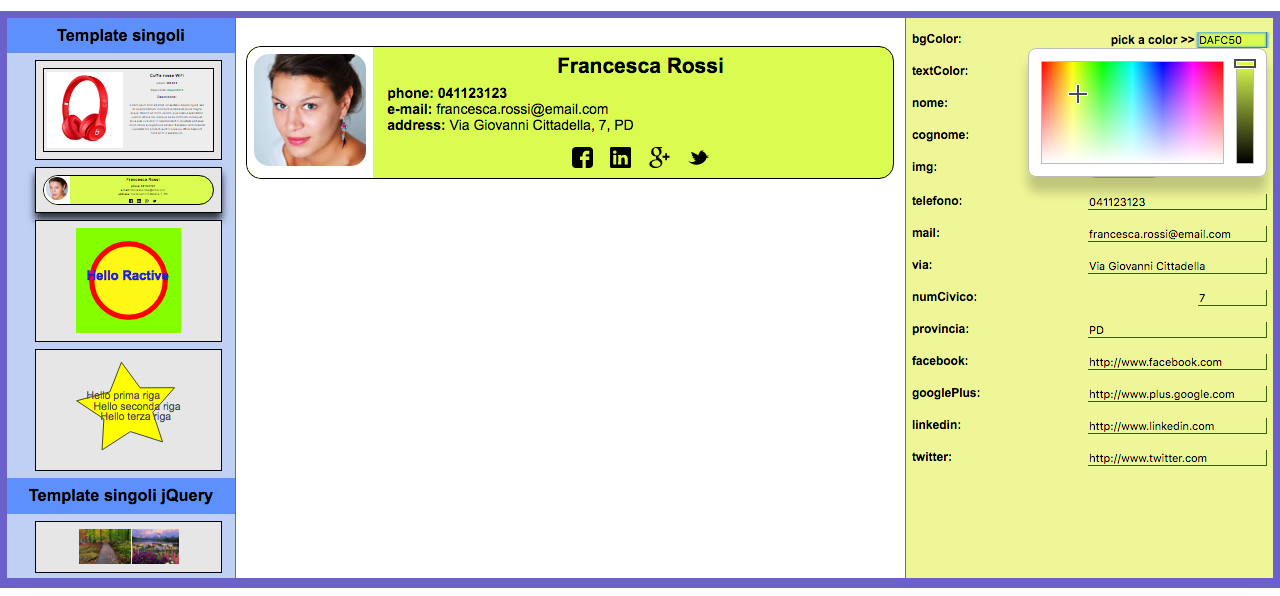
\includegraphics[scale=0.32]{../immagini/screenshot_app}
	\caption{Screenshot dell'applicazione realizzata.}
\end{figure}
I risultati ottenuti dallo studio delle librerie e l'applicazione realizzata soddisfano le aspettative dell'azienda.\\
La fase di prototipazione dei template, utilizzando la libreria \textit{Ractive.js}, ha messo in evidenza le potenzialità offerte da questo strumento e ha permesso all'azienda di trovare vari modi per sfruttare la libreria nello sviluppo dei loro prodotti.\\
Le richieste relative ai template sono state soddisfatte, dimostrando che è possibile creare template che si comportino in modo responsive e che integrino plug-in JQuery senza grandi sforzi da parte dello sviluppatore.\\
Il funzionamento dei template in ambito mobile è stato possibile tramite l'aggiunta del plug-in \textit{ractive-events-tap} che permette di gestire in maniera appropriata il tap su di un touchscreen.\\
Inoltre la possibilità di inserire il codice di attivazione per i plug-in JQuery all'interno della logica del template ne assicura la corretta esecuzione.\\
Per quanto riguarda i risultati ottenuti con l'applicazione, questi sono stati soddisfacenti per l'azienda, in quanto l'applicazione si comporta come era stato richiesto offrendo la possibilità di selezione e visualizzazione dei vari template e di modifica dei dati ad essi relativi.\\
Lo scopo principale dell'applicazione realizzata è stato quello di evidenziare le possibilità di integrazione della libreria \textit{Ractive.js} all'interno di un web application e di fornire un punto di partenza per lo sviluppo di un'eventuale estensione per l'applicativo aziendale \textit{Portal Studio}.
 
\subsection{Requisiti soddisfatti}
%RFF1.1.1 RFF2.1 RVF10
\section{Criticità}

\section{Conoscenze acquisite}
